\section{Systematics}
\label{sec:systematics}


% \subsubsection{Background systematics}
%
% Systematic uncertainties on the transfer factors are determined from
% closure tests in data as a function of \njet and regions in
% \scalht. These uncertainties are assumed to be fully correlated
% between \scalht bins within a region, and fully uncorrelated between
% \scalht regions and (\njet,\nb) categories, as done during Run~1. In
% the absence of biases, the systematic uncertainties are statistically
% limited by the control sample yields. 
%
% Estimates based on the values obtained for the Run~1 analyses while
% extrapolating to the higher cross sections expeced in Run~2, and
% accounting for the finer categorisation of events in the signal region
% and control samples, are shown in Table~\ref{sec:bkgd-syst}.
%
% \begin{table}[h!]
%   \caption{Systematic uncertainties on the transfer factors as a
%     function of \scalht.}  
%   \label{tab:bkgd-syst}
%   \setlength{\extrarowheight}{2.5pt}
%   \centering
%   \begin{tabular}{ llccc }
%     \hline
%     \hline
%     \scalht region [GeV] & 200-600 & 600-1000  & $>1000$  \\ 
%     \hline
%     Uncertainty [\%] & 10 & 20 & 30 \\
%     \hline
%     \hline
%   \end{tabular}
% \end{table}
%
% The uncertainties associated with the b-tag ``fomula method'' used
% during Run~1 are ascertained through a dedicated procedure and are
% assumed to be sub-dominant with respect to the \scalht-dependent
% uncertainties derived from the closure tests, as observed during
% Run~1. 
%\clearpage

\section{Closure tests and systematic uncertainties on transfer factors\label{sec:bkgd-syst}}

The normalisation of the \mht dimension in the signal region is determined from 
a transfer factor from control regions as described in \ref{sec:background}. 
An appropriate systematic uncertainty is assigned to each factor to
account for theoretical uncertainties~\cite{Bern:2011pa} and
limitations in the simulation modelling of event kinematics and
instrumental effects. This section describes how the systematic
uncertainties are determined from closure tests in data.

\subsection{Closure tests\label{sec:closure-tests-desc}}

The sensitivity of the transfer factors to potential limitations in
the simulation modelling is established through sets of closure tests,
which confront data yields measured in one data control (sub-)sample
against the predictions determined from another data control
(sub-)sample as a function of \scalht. \ie, an extrapolation is made
from one control (sub-)sample to another (rather than to the signal
region) in bins of \scalht via appropriate transfer factors, again
determined from simulation. A large ensemble (\ie hundreds) of
statistically independent closure tests are performed between a number
of control (sub-)samples to identify any potential sources of bias in
the transfer factors.

The level of statistical consistency between the predicted and
observed yields of each closure test in the ensemble is inspected, in
the absence of any assumed systematic uncertainty. The level of
agreement between the predicted and observed yields is expressed as
the ratio $(\nobs - \npre)/\npre$ while considering only the
statistical uncertainties on \npre and \nobs. Therefore, the level of
closure is defined by the statistical significance of a deviation in
the ratio from zero. A set of closure tests comprise ratios determined
for each \scalht bin. In this way, a set of closure tests allow to
establish the presence of significant biases or otherwise, and any
possible dependence on \scalht. If statistically significant biases
are observed, further studies are required to understand and correct
for these biases.

Under the assumption of closure for the full ensemble of tests,
systematic uncertainties on the transfer factors are derived for each
\njet and \nb category and \scalht regions. The treatment for
estimating the systematic uncertainties on the transfer factors is
described in Section~\ref{sec:syst-from-closure}.

Eight sets of closure tests use the five data control samples to
probe key ingredients of the simulation modelling of the SM
backgrounds with genuine \met as a function of \scalht, as shown in
Fig.~\ref{fig:closure}. This is done for each jet multiplicity bin
separately: 

\begin{figure}[h!]
  \begin{center}
    \subfigure[$2 \leq \njet \leq 3$]{\includegraphics[width=0.7\textwidth]{figures/syst/v0/le3j/summary_plot}} \\
    \subfigure[$\njet \geq 4$]{\includegraphics[width=0.7\textwidth]{figures/syst/v0/ge4j/summary_plot}} \\
    \caption{PLACEHOLDER Sets of closure tests (open symbols) overlaid on top of
      the systematic uncertainty used for each of the five \scalht
      regions (shaded bands) and for the two different jet
      multiplicity bins: (a) $2 \leq \njet \leq 3$ and (b) $\njet \geq
      4$.  }
    \label{fig:closure}
  \end{center} 
\end{figure}

The first three sets of closure tests are carried out between the $\mu$ 
+ jets sample and the e + jets sample. These probe the lepton 
identification for three background scenarios. These are 0 (red circles), 
1 (times symbols) and $\ge2$ (squares) b-jets and probe lepton identification 
for W, W + \ttbar and \ttbar respectively.
% The first three sets of closure tests are carried out within the $\mu$
% + jets sample. The first set (indicated by circles) probes the
% modelling of the \alphat distribution in genuine \met events as a
% function of \scalht. This is important to verify the approach of using
% \mj and \mmj samples without an \alphat requirement to make background
% predictions in the signal region, as described in
% Sec.~\ref{sec:larger}. The tests confront data yields in the \mj
% sample with an \alphat requirement against predictions determined in a
% \mj sample with the \alphat requirement inverted. As usual,
% corresponding expectations from simulation are obtained to construct
% the transfer factors required to make the predictions.

The fourth (triangles) and fifth (green crosses) sets probe the
sensitivity of the transfer factors to the relative admixture of
events from the $W$ + jets and \ttbar processes. These tests are
extremely conservative, as the admixture changes little between the
\mj sample and the signal region, whereas the closure tests use
sub-samples with very different admixtures of W + jets and \ttbar
events. \eg, the former uses a W-enriched sub-sample (selected by
requiring zero b-jets) to predict yields in a \ttbar-enriched
sub-sample (selected by requiring one b-jet). These two tests also
probe the modelling of the reconstruction of b-quark jets, although
this is also addressed more fully by dedicated studies that determine
systematic uncertainties via the method described in
Sec.~\ref{sec:btag-syst}.

The sixth (hollow stars) and seventh (inverse triangles) set deals 
with the consistency of the prediction of W + jets with $\gamma$ + jets.
This is useful in general for understanding the predictions of vector 
bosons (\ie \znunu + jets) from the \gj process. 


The eigth (diamonds) and ninth (brown asterix), connecting the $\mu$ + jets 
and $\mu\mu$ + jets control samples, again addresses the modelling of 
the relative contributions of $Z$ + jets to $W$ + jets and \ttbar events.
This set of tests is again a very conservative probe of the sensitivity of the
transfer factors to the W + jets and \ttbar admixture. At some
level, the muon trigger and reconstruction efficiencies are probed
too, given that exactly one and two muons are required in the two
control samples. However, dedicated data-driven methods are used to
measure the muon trigger and reconstruction efficiencies, with values
taken from the muon POG.

The tenth (solid stars) and eleventh (red crosses) deals with the consistency between the
Z$\rightarrow\mu\mu$ + jets and $\gamma$ + jets samples, which is an
important self-consistency cross-check between two independent methods
used to predict the same irreducible background of \znunu + jets
events. Hence, this is also an important check on the validity of
using the \gj process to predict the \znunu\, + jets process.
%, for which a 20\% theoretical uncertainty on the ratio of
%cross-sections is assumed~\cite{PAS-SUS-08-002,Bern:2011pa}.

The twelth, and thirteenth tests probe the simulation modelling of
the jet multiplicity in the e + jets (green asterix), and ee + jets 
(blue circles), which is checked due to the exclusive binning in jet multiplicity.
As in the case of the W + jets / \ttbar admixture, this set of tests is a very 
conservative check, as predictions are always made from the same 
jet multiplicity bin, whereas the closure tests translate between the two bins.

% This section assumes data - must alter to what we show
In summary, each set of closure tests should demonstrate, within the
statistical precision of each test, that there are no significant
biases or dependencies on \scalht inherent in the transfer factors
obtained from simulation. To ensure this zero and first order polynomial
fits will be performed along the \scalht dimension for each closure test 
and jet category. The fits will be inspected for any indication of bias 
averaged over \scalht as well as a bias dependant on \scalht. 

\subsection{Systematic uncertainties from closure tests\label{sec:syst-from-closure}}

Once it is established that no significantly large bias or trend is
observed for any set of closure tests the systematic uncertainties
are determined. The statistical precision of the closure tests is
considered a suitable benchmark for determining the systematic
uncertainties that are assigned to the transfer factors, as it is only
the statistical uncertainties associated with the tests that limit our
knowledge of whether closure is actually achieved or otherwise.

Expected systematics are determined for seven regions in \scalht,
for each jet category as indicated in Figure~\ref{fig:doesntexist}. 
A missing entry implies that the statistics were insufficient to complete
the necessary set of closure tests and the \scalht bin is not used 
for this jet category. In data for each \scalht region, the systematic uncertainty 
is estimated by taking the quadrature sum of the weighted mean and sample variance for 
the closure tests within the given \scalht region. To find expected systematics the weighted 
mean of the closure tests errors is used as an estimator of the expected variance.
This procedure yields the values quoted in Figure~\ref{fig:doesntexist}. In addition to 
the fits described in \ref{sec:systematics} comparing the size of the systematic found
in data with that expected will provide an indication of bias.

The effect of uncertainties related to the modelling of b-quark jets
in simulation on the transfer factors is found to be negligible, at
the percent level as discussed in Section~\ref{sec:btag-syst}, in
comparison to the aforementioned \njet- and \scalht-dependent
systematic uncertainties.

\begin{table}[!h]
  \caption{A summary of the magnitude of the systematic uncertainties (\%)
    assigned to the transfer factors, according to \njet and \scalht
    region.}
  \label{tab:syst-values}
  \centering
  \footnotesize
  \begin{tabular}{ cccccccc }
    \hline
    \hline
            & \multicolumn{7}{c}{\scalht region (GeV)}                                \\
    \cline{2-8}
    \njet   & 200--275 & 275--325 & 325--375 & 375--575 & 575--775 & 775-975 & $>975$ \\
    \hline                                                                                                                                  
    2--3    & 4        & 6        & 6        & 8        & 12       & 17      & 19     \\
    $\geq$4 & 6        & 6        & 11       & 11       & 18       & 20      & 26     \\
    \hline                                                                                                                                  
    \hline
  \end{tabular}
\end{table}

Figure~\ref{fig:closure} shows the sets of closure tests overlaid on
top of grey bands that represent the \scalht-dependent systematic
uncertainties in Table~\ref{tab:syst-values}. These systematic
uncertainties are assumed to fully uncorrelated between the different
b jet multiplicity categories and also the seven \scalht regions,
which is a conservative approach given that one can expect some
correlation between adjacent \scalht bins (due to comparable
kinematics).  This approach of decorrelating the \scalht regions
should be contrasted against the fits shown in
Figure~\ref{fig:closure-fits} that do assume a correlated behaviour in
\scalht.
% while some fits outside bands, could argue to use correlation. plus
% fit uncertainties not shown. 

%\subsection{Conservative closure tests and systematic uncertainties\label{sec:conservative}} 
%
%As mentioned briefly above, several sets of closure tests are
%considered to be very conservative, due to the significant differences
%in background composition and event kinematics between the two
%sub-samples used in the closure test relative to the (much smaller)
%differences between each control sample and the corresponding
%background(s) in the signal region. The accurate mirroring of the
%signal region and control samples is due to kinematically-similar
%event selections and the fact that the predictions are always made
%using the same (\njet, \nb, \scalht) bin. Conversely, suitable
%examples of conservative closure tests are: the two tests that change
%the \nb requirement (within the \mj sample), the test that uses the
%\mj and \mmj samples, and the three tests that change the \njet
%requirement (for each control sample).
%
%Consequently, the systematics derived from these conservative closure
%tests are also considered to be conservative. One important test of
%this statement is the sensitivity of the transfer factors to the
%admixture of W + jets and \ttbar in the signal region and \mj control
%sample. This is demonstrated by Fig.~\ref{fig:vary-xs-le3j} in
%Appendix~\ref{app:vary-xs}, which shows the effect of varying the
%cross sections of the W + jets and \ttbar by by $+$20\% and $-$20\%,
%respectively, on the closure tests performed in the \njet multiplicity
%bin \njetlow. Similarly, Fig.~\ref{fig:vary-xs-ge4j} shows the effect
%in the \njet multiplicity bin \njethigh. This variation in cross
%sections (in opposite directions) is considered to be extreme and is
%motivated (loosely) by the uncertainty on the experimental
%measurements of the W + jets and \ttbar inclusive cross sections.
%
%Given these variations in cross sections, the level of closure for
%several tests is subsequently degraded significantly and introduces
%apparently significant biases. However, the effect on the transfer
%factors used in the analysis (to ``translate'' an observation in a
%control sample to a prediction in the signal region) is negligible due
%to the ``mirroring'' of the signal region and control
%samples. Table~\ref{tab:vary-xs} demonstrates this by showing the
%effect on the transfer factors used to predict the W + jets and
%\ttbar backgrounds when varying the cross sections of W + jets and
%\ttbar by $+$20\% and $-$20\%, respectively. (In this case, no
%requirement is made on \njet, but the same behaviour is observed for
%the exclusive \njet bins.) While the artificial biases introduced to
%the closure tests are as large as $\sim$30\%, most apparent in the
%lowest \scalht bins, the effect of the transfer factors used in the
%analysis is typically at the percent level and only as large as
%$5\%$. 
%
%Hence, given the robust behaviour of the transfer factors with
%respect to large (and opposite) variations in the W + jets and \ttbar
%cross sections, one can assume with confidence that any bias in the
%transfer factors is adequately (and conservatively) covered by the
%systematic uncertainties -- of at least 10\% -- used in the analysis.

%%____________________________________________________________________________||
